\section{Exigences typiques et considérations de conception}
Pour la mission spatiale, le système de communication doit être conçu pour répondre aux besoins de liaison montante et descendante des données de la charge utile et du bus du vaisseau spatial. Les exigences comprennent des spécifications techniques pour :
\begin{itemize}
\item Avant tout, le système de communication dans son ensemble doit avoir un bilan de liaison qui se ferme et, de manière optimale, présente une marge positive.
\begin{itemize}
\item Les principaux facteurs qui influencent le bilan de liaison sont la puissance disponible pour la transmission, le gain de l'antenne (géométrie et masse), la température des composants et l'orbite (pertes). Ces paramètres seront développés dans la section sur les bilans de liaison.
\item Les pertes du système proviennent de la température des composants. Le sous-système thermique peut devoir respecter les exigences imposées par le sous-système de communication.
\end{itemize}
\begin{figure}[H] % H force l'affichage ici
    \centering
    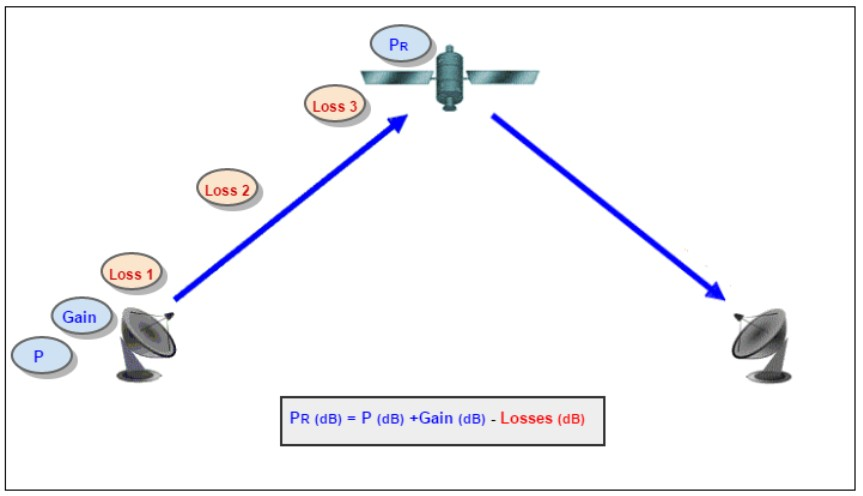
\includegraphics[width=0.8\textwidth]{figures/6-6.jpg}
        \caption{Gain de l'amplificateur de l'émetteur et du récepteur. Atténuation dans la propagation dans l'atmosphère. Pertes de dépointage. Pertes dues à la désadaptation de polarisation. Pertes dans les équipements de transmission et de réception. Image de Source Forge.}
    \label{fig:communication2}
\end{figure}
\item Débit de données entre le vaisseau spatial et la station au sol pour la transmission des données de charge utile et la transmission des commandes ou des logiciels d'opération de mission. Cette mesure ressemble beaucoup à l'exigence de débit du CDH, mais au lieu de l'interface entre la charge utile et l'ordinateur de vol, le débit de données est l'interface entre le vaisseau spatial et la station au sol.
\item Le temps de contact avec les stations terrestres (et le débit de données) détermine le nombre total de données qu'un vaisseau spatial est capable de transmettre. Le temps de contact dépend du nombre et de l'emplacement des stations terrestres, ainsi que de l'orbite du vaisseau spatial.
\begin{itemize}
\item Étant donné que le vaisseau spatial peut communiquer avec le sol, la charge utile génère une certaine quantité de données qui sont nécessaires à la transmission en liaison descendante pour remplir la mission. Cette exigence de niveau supérieur contribue aux exigences de débit de données et de temps de contact.

\end{itemize}
\begin{figure}[H] % H force l'affichage ici
    \centering
    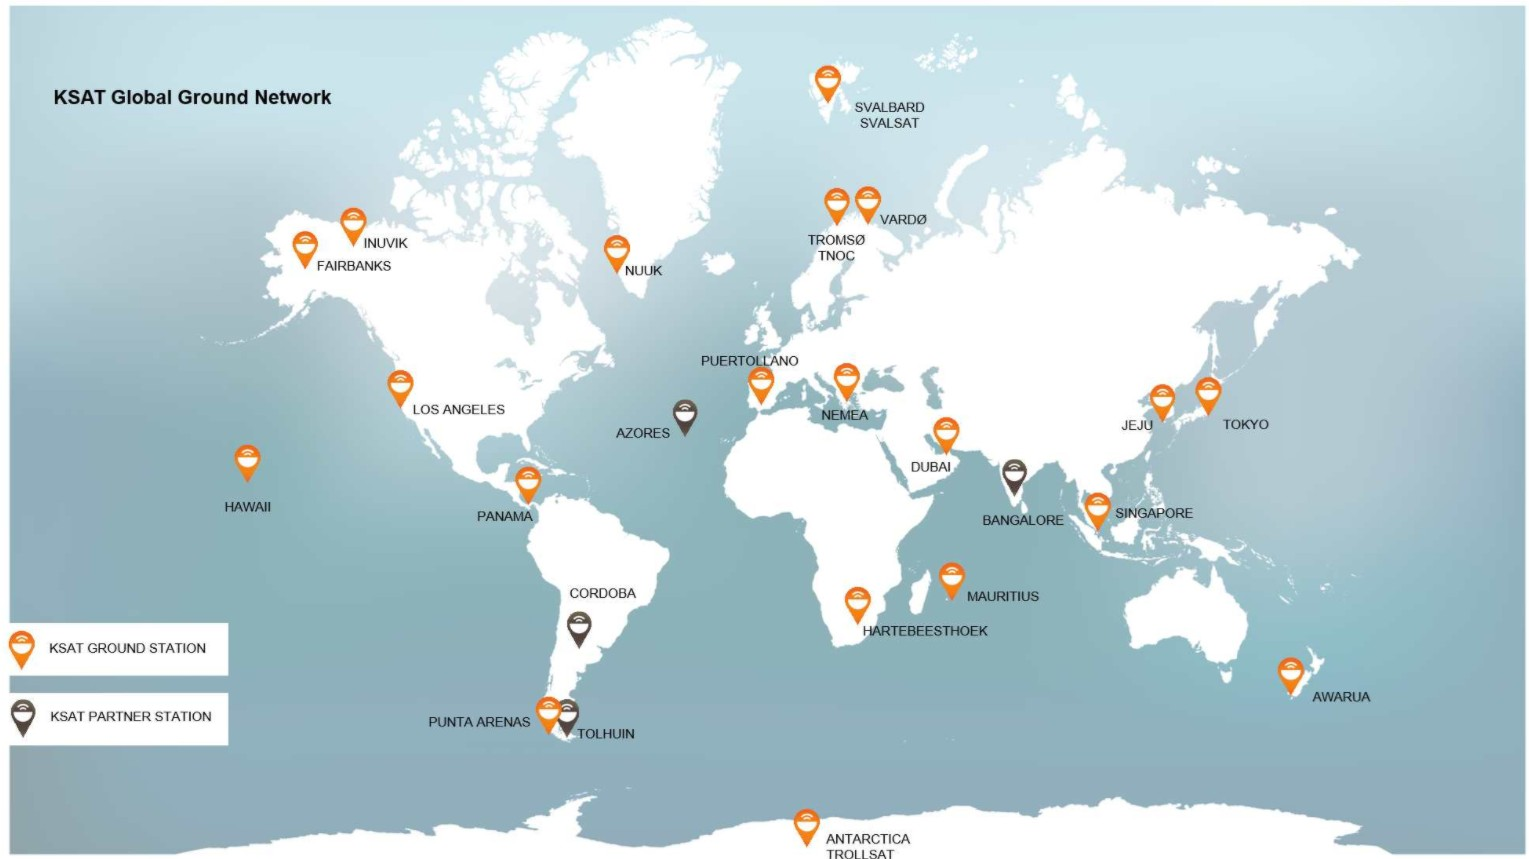
\includegraphics[width=0.8\textwidth]{figures/6-7.jpg}
    
    \caption{KSAT vous donne accès à notre vaste réseau terrestre mondial composé de stations situées aux deux pôles et à des emplacements triés sur le volet à moyenne latitude pour garantir un accès continu à vos satellites. Image de KSAT.}
    \label{fig:communication2}
\end{figure}
\item La directionnalité (omnidirectionnelle ou directionnelle) de l'antenne détermine l'obligation du système de détermination et de contrôle d'attitude de pointer le vaisseau spatial pendant les communications. Cette manœuvre de pointage affecte également la manière dont nous effectuons les opérations de mission.
\begin{figure}[H] % H force l'affichage ici
    \centering
    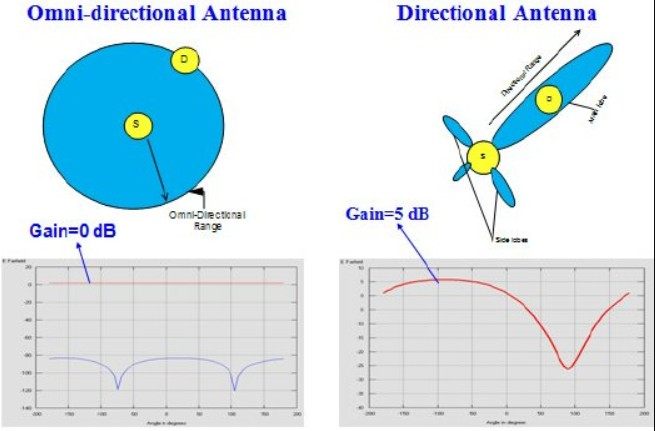
\includegraphics[width=0.8\textwidth]{figures/6-8.jpg}
    \caption{Diagrammes de rayonnement des antennes omnidirectionnelles et directionnelles.}
    \label{fig:communication2}
\end{figure}
\item Le chercheur principal peut imposer une quantité suffisante de bruit ou de perte de signal. Le spécialiste des communications doit alors tenir compte de ce bruit ou de cette perte dans la conception du codage et de la modulation.
\end{itemize}
\textbf{Documents requis}
\begin{itemize}
    \item La spécification de conception CubeSat Rev. 14 impose des exigences en matière de licences radio :
    \begin{itemize}
        \item \textbf{Obtention des licences} :
        \begin{itemize}
            \item Les opérateurs doivent obtenir et fournir la documentation relative aux licences appropriées pour l’utilisation des fréquences radio.
            \item \textit{Remarque} : Pour l'utilisation de fréquences amateurs, il faut prouver que la fréquence a été coordonnée par l'IARU. Les demandes peuvent être consultées sur \url{https://www.iaru.org}.
        \end{itemize}
        \item \textbf{Conformité aux réglementations nationales} :
        \begin{itemize}
            \item Les CubeSats doivent respecter les accords et restrictions de licence radio de leur pays.
            \item \textit{Remarque} : Les opérateurs CubeSat doivent se référer à l'Union internationale des télécommunications (UIT) pour déterminer les licences et les approbations nécessaires pour leur pays.
        \end{itemize}
    \end{itemize}
\end{itemize}
\begin{itemize}
    \item Le temps entre le déploiement et la transmission par radiofréquence est exigé en externe par les fournisseurs de lancement.
    \begin{itemize}
        \item L'IDD du déployeur CubeSat externe NanoRacks spécifie dans les commutateurs de déploiement:
        \item 4.1.4-5) Les commutateurs de déploiement du CubeSat doivent réinitialiser la charge utile à l'état de pré-lancement s'ils sont actionnés à tout moment dans les 30 premières minutes après la fermeture des commutateurs (y compris, mais sans s'y limiter, la transmission radiofréquence et les minuteries du système déployable).
     \end{itemize}
    \item Le nombre de stations terrestres auxquelles vous avez accès et le niveau d'accès dont vous disposez. À moins que vous n'ayez construit votre propre station terrestre, vous devrez probablement utiliser la station terrestre ou le réseau de quelqu'un d'autre. Travailler avec d'autres personnes comporte des contraintes qui dépendent de leur disponibilité, de leur coût et de votre relation avec l'organisme de contrôle.
    \begin{itemize}
        \item Réseau de stations terrestres internationales (IGS) exploité par notre réseau de stations terrestres américaines et internationales (IC).
        \item Station terrestre Amazon Web Services sous Amazon.
        \item SatNOGS, un réseau mondial open source de stations terrestres par satellite, détenu et exploité par la communauté.
    \end{itemize}
\end{itemize}
\begin{figure}[H] % H force l'affichage ici
    \centering
    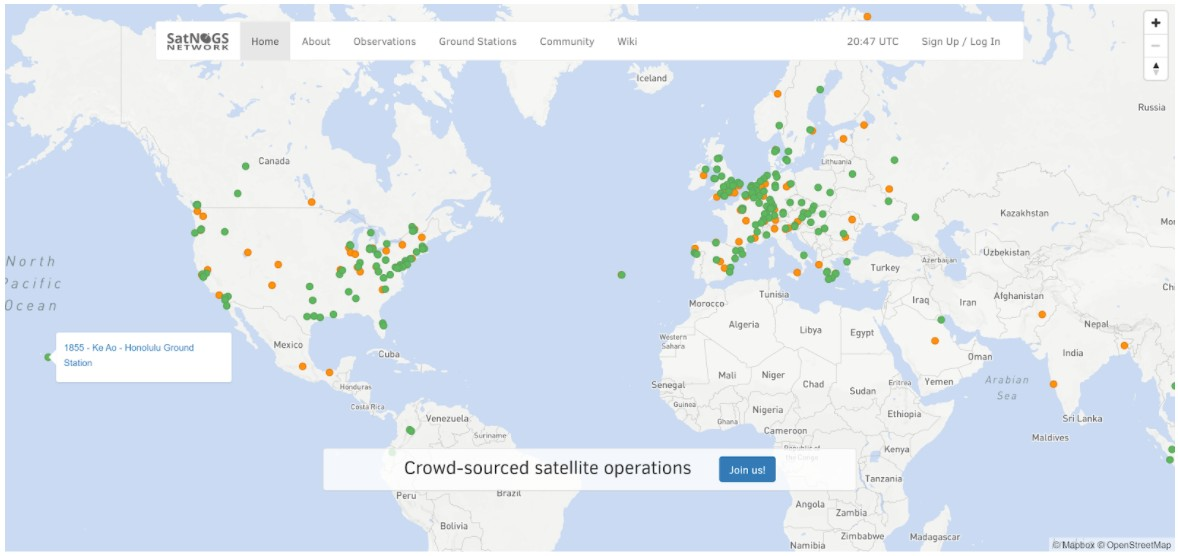
\includegraphics[width=0.8\textwidth]{figures/6-10.jpg}
    
    \caption{Réseau SatNOGS actuel au 17/12/2020 à 10h47 HST. Image de Satnogs Network.}
    \label{fig:communication2}
\end{figure}
Lors de la fabrication et de l'assemblage, vous, en tant que spécialiste des communications, devez manipuler plusieurs composants, allant de la carte de communication à l'antenne, en passant par les amplificateurs, les radios, etc. Vous travaillerez probablement avec le spécialiste des systèmes d'alimentation, car le système de communication est gourmand en énergie. La manipulation des systèmes de communication suit les meilleures pratiques des composants des systèmes d'alimentation électrique.
\begin{figure}[H] % H force l'affichage ici
    \centering
    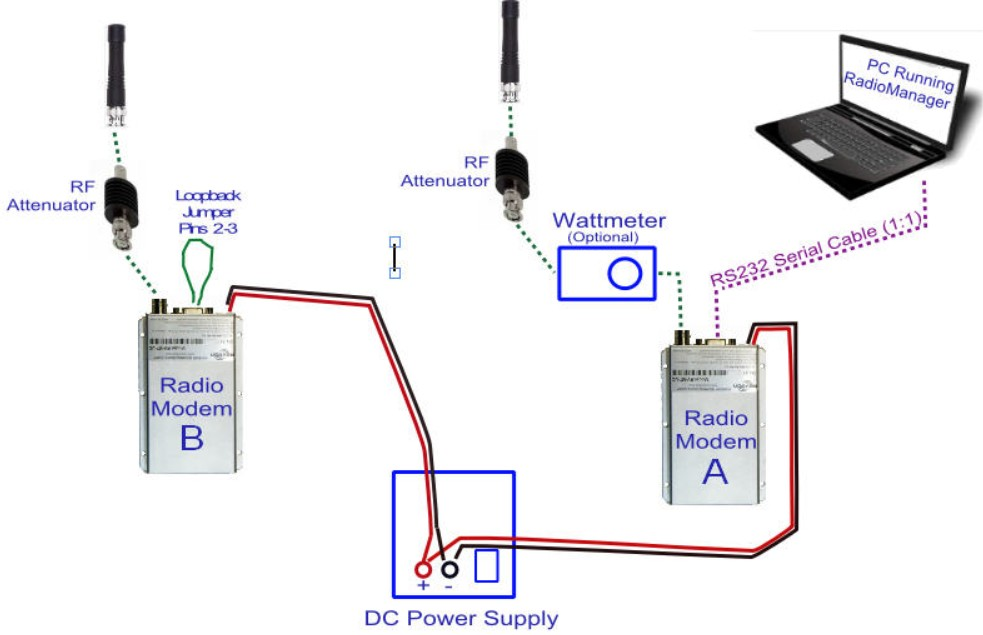
\includegraphics[width=0.8\textwidth]{figures/6-11.jpg}
    
    \caption{Test radio en plein air ou test de liaison, qui effectue les opérations suivantes : Capture de la configuration/des paramètres du modem radio dans un fichier. Vérification que le modem radio transmet le niveau de puissance de sortie RF correct. La fréquence du modem radio est correctement définie. Les paramètres du port série sont corrects. Le débit en bauds en direct est correct et compatible avec le système dans lequel le modem sera utilisé. Vérification et enregistrement de la consommation d'énergie CC. Détermination du taux d'erreur de paquets sur le banc ou sur le terrain. Image de Raveon.}
    \label{fig:communication2}
\end{figure}

Lors des tests, le logiciel de codage et de modulation doit être chargé et testé avec le matériel. Pour vérifier les communications de bout en bout entre la radio du vaisseau spatial et votre récepteur, une distance appropriée est placée entre la radio et le récepteur, et les pertes qui se produiraient entre l'espace et le sol sont simulées par des atténuateurs, fixés à chaque extrémité [ NASA MAVEN ]. Les signaux sont surveillés sur un ordinateur pour voir 1) si les signaux sont captés et 2) la quantité de perte dans les signaux reçus. L'intégration de ce code dans le logiciel général du vaisseau spatial impliquera le spécialiste du commandement et du traitement des données.

Pendant le transport et la manutention, l'ordinateur de vol est éteint et autonome dans le satellite. Le spécialiste des communications n'a aucune exigence à respecter à ce stade.
\begin{figure}[H] % H force l'affichage ici
    \centering
    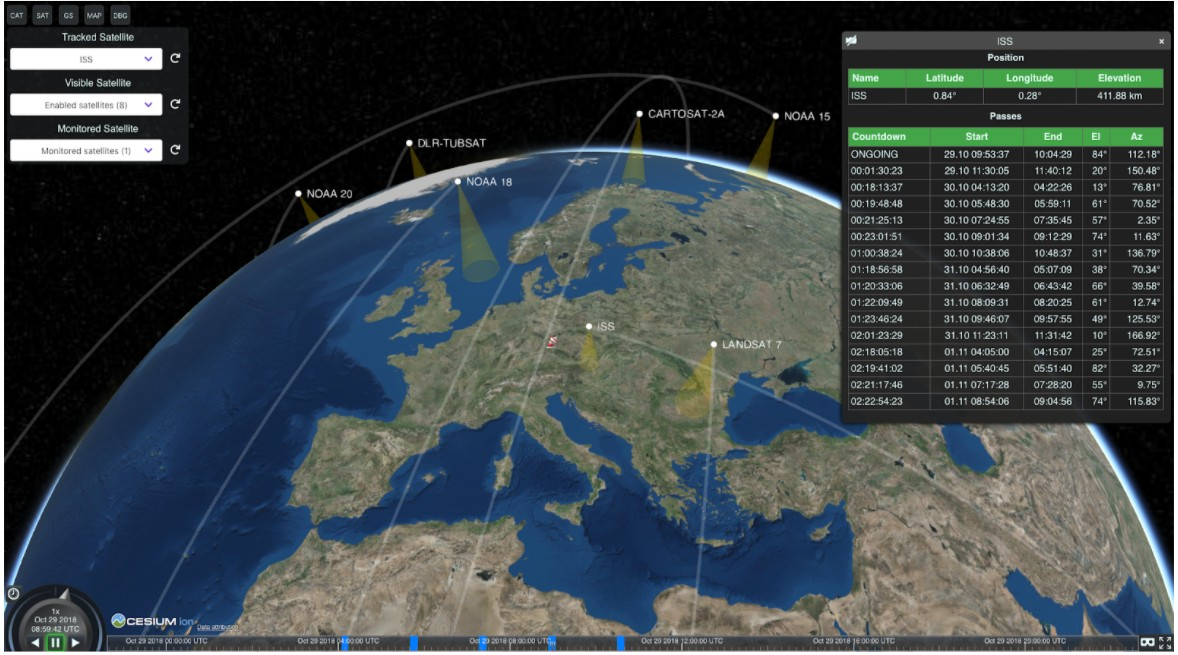
\includegraphics[width=0.8\textwidth]{figures/6-12.jpg}
    
    \caption{Visualisation de l'orbite des satellites et prédiction de leur passage. Image de Florian Mauracher sur Github.}
    \label{fig:communication2}
\end{figure}
Depuis la livraison jusqu'au déploiement en orbite, le spécialiste des communications doit s'assurer que le logiciel de suivi d'orbite et de station au sol est prêt à fonctionner. Une fois le vaisseau spatial déployé, le spécialiste des communications doit mettre à jour les éléments orbitaux (TLE ) dans son logiciel de station au sol afin que la station au sol directionnelle puisse s'orienter avec précision dans la direction du vaisseau spatial. Pour les stations au sol omnidirectionnelles ou directionnelles, la mise à jour des TLE informera les opérateurs de mission du moment où le vaisseau spatial passe au-dessus de leur tête dans une zone de portée communicable.
\begin{center}
    \textbf{Kit Artemis spécifique}
\end{center}
\begin{itemize}
    \item \textbf{Système de communication CubeSat} :
    \begin{itemize}
        \item Le système de communication CubeSat transmettra la télémétrie depuis l'orbite terrestre basse (LEO).
        \item \textbf{Exigences de transmission} :
        \begin{itemize}
            \item La radio doit transmettre une télémétrie détectable en fréquence radio amateur (UHF).
            \item Les stations au sol recevront le signal UHF et traiteront la télémétrie réelle.
            \item Le bilan de liaison doit avoir une marge d'au moins 5 dB.
        \end{itemize}
    \end{itemize}
\end{itemize}
\begin{center}
    \textbf{Activité suggérée}
\end{center}
« Quelles exigences de communication devez-vous imposer à votre système pour remplir votre mission scientifique ? »
 



